%*****************************************
\chapter{Thematic Coherence in Fake News}\label{ch:thematic-coherence}
%*****************************************

\setcounter{hyp}{-1}

\section{Background}
\label{sec:4-background}

This\sidequote{The construction of life is at present in the power far more of facts than of convictions, and of such facts as have scarcely ever become the basis of convictions.}{Walter Benjamin}{https://doi.org/10.2307/j.ctvjk2x1m.5}{One-Way Street} chapter deals with the exploration of thematic coherence of fake news. News readers are often enticed by the headlines of articles, or their opening sentence(s). False news is written for many different reasons, including propaganda, provocation and profit,\sidecite{Shu:2017} and therefore, often in catchy or emotive language. Given the deluge of information which competes daily for people's attention, most people would now skim through news pieces that they would otherwise carefully read—perhaps to save their time—or in an attempt to spend it on stories of greater interest to them. However, this inattention can be exploited by propagators of misinformation, as they can make the headlines or openings of false news captivating. An indication of a misleading article could, therefore, be that its headline or starting paragraph thematically deviates from the rest of the article.

In this chapter, the focal point is fake news that appears in the form of long online articles and explores the extent of internal consistency within fake news vis-à-vis legitimate news. In particular, these experiments aim to determine whether \emph{thematic deviations}—\emph{i.e.}, a measure of how dissimilar topics discussed in different parts of an article are—between the opening and remainder sections of texts can be used to distinguish between fake and real news across different news domains. Put simply, this is a measure of the distance between the distributions of topics extracted from two sections of an article, the opening and the remainder. The dissemination of fake news is increasing, and because it appears in various forms and self-reinforces,\sidenote{\citeauthoryear{Wardle:2017}, \citeauthoryear{Waldman:2018}, \citeauthoryear{Zhou:2018}} it is difficult to erode. Hence, there is an urgent need for increased research in understanding and curbing it.

\newthought{One study by} \citeauthoryear{Gabielkov:2016} found that, as of 2016, 59\% of links shared on OSNs have never been clicked before. This indicates that people share information without actually reading it. A more recent study by \citeauthoryear{Anspach:2019} suggests that some readers may skim through an article instead of reading the whole content because they overestimate their political knowledge, while others may hastily share news without reading it fully, for emotional affirmation. This presents bad actors with the opportunity to deftly intersperse news content with falsity. Moreover, the production of fake news typically involves the collation of disjointed content and lacks a thorough editorial process.\sidecite{Karimi:2019} The limitation of existing misinformation detection methods not adequately capturing the subtle differences between false and legitimate news motivates the experiments presented in this section.

\newthought{Topics discussed in} news pieces can be studied to ascertain whether an article \emph{thematically deviates} between its opening and the rest of the story, or if it remains coherent throughout. In other words, does an article open with one topic and finish with a different, unrelated topic? Thematic analysis is useful here for two reasons. First, previous studies show that the coherence between units of discourse (such as sentences) in a document is useful for determining its veracity.\sidenote{\citeauthoryear{Rubin:2015}, \citeauthoryear{Karimi:2019}} Second, analysis of thematic deviation can identify general characteristics of fake news that persist across multiple news domains.

Topics have been employed as features for misinformation detection using \ac{ML}.\sidenote{\citeauthoryear{Bhattacharjee:2018}, \citeauthoryear{Benamira:2019}, \citeauthoryear{Li:2019}} However, they have not been applied to study the unique characteristics of fake news. Research efforts in detecting fake news through thematic deviation have thus far focused on spotting incongruences between pairs of headlines and body texts.\sidenote{\citeauthoryear{Chen:2015}, \citeauthoryear{Ferreira:2016}, \citeauthoryear{Sisodia:2019}, \citeauthoryear{Yoon:2019}} Yet, thematic deviation can also exist within the body text of a news item. The focus is to examine these deviations to distinguish fake from real news.

To the best of the author's knowledge, this is the first work that explores thematic deviations in the body text of news articles to distinguish between fake and legitimate news.

\section{Related work}
\label{sec:4-related-work}

The coherence of a story may be indicative of its veracity. For example, \citeauthoryear{Rubin:2015} demonstrated this by applying \ac{RST}\sidecite{Mann:1988} to study the discourse of deceptive stories posted online. They found that a major distinguishing characteristic of deceptive stories is that they are disjunctive. Furthermore, while truthful stories provide evidence and restate information, deceptive ones do not. This suggests that false stories may tend to thematically deviate more due to disjunction, while truthful stories are likely to be more coherent due to restatement. Similarly, \citeauthoryear{Karimi:2019} investigated the coherence of fake and real news by learning hierarchical structures based on sentence-level dependency parsing. Their findings also suggest that fake news documents are less coherent.

\newthought{Topic models are} unsupervised algorithms that aid the identification of themes discussed in large corpora. With them, these texts can be understood, organized, summarised and searched for automatically.\sidecite{Blei:2012} One example of topic models is \ac{LDA}, which is a generative probabilistic model that aids the discovery of latent themes or \emph{topics} in a corpus.\sidecite{Blei:2003} \citeauthoryear{Vosoughi:2018} used \ac{LDA} to show that false rumour tweets tend to be more novel than true ones. Novelty was evaluated using three measures: Information Uniqueness, Bhattacharyya Distance, and Kullback-Leibler Divergence. Likewise, \citeauthoryear{Ito:2015} used \ac{LDA} to assess the credibility of Twitter users by analyzing the topical divergence of their tweets from those of other users. They also assessed the veracity of users’ tweets by comparing the topic distributions of new tweets against historically discussed topics. Divergence was computed using the Jensen-Shannon Divergence, Root Mean Squared Error, and Squared Error. This work primarily differs from those two, in that here, full-length articles are analysed instead of tweets.

\section{Problem definition}
\label{sec:4-problem}

Building on the previous subsections, the aim is to establish whether or not there is evidence to distinguish between fake and authentic news, based on the coherence of topics discussed in them. Similar to \autoref{ch:word-embeddings}, the statistical hypothesis testing approach is found to be appropriate for carrying out this study. The following hypotheses are tested:

\begin{hyp}
  [Null] \label{hyp:a}\textit{False and authentic news articles are similarly coherent thematically.}
\end{hyp}
\begin{hyp}
  [Alternative] \label{hyp:b}\textit{the thematic coherence of authentic news articles is greater than that of false news articles.}
\end{hyp}

Specifically, the thematic drift between the opening part and the remaining part of an article is measured, to see how they differ. The primary tool used to measure this is \ac{LDA} topic modelling.
 The opening section of an article is defined using a hyperparameter, $l$, which is the number of sentences at the start of it. To test \Cref{hyp:a,hyp:b}, experiments are carried out in the manner outlined in Algorithm \autoref{4-divergence}. The differences in mean and median coherence values of fake and real articles are evaluated using an Independent Samples T-test, at 5\% significance level.

\section{Research Goal and Contributions}
\label{sec:4-goals-contributions}

The research presented in this chapter aims to assess the importance of internal consistency within articles as a high-level feature to distinguish between fake and real news stories across different domains. This chapter sets out to explore whether the opening segments of fake news thematically deviate from the rest of it, significantly more than in authentic news. Experiments are conducted using seven datasets which collectively cover a wide variety of news domains, from business to celebrity, to warfare. Deviations are evaluated by calculating the distance between the topic distribution of the opening part of an article, to that of its remainder. The first five sentences of an article are taken as its opening segment.

The following summarise the contributions of this chapter:

\begin{itemize}
  \item It presents new insights towards understanding the underlying characteristics of fake news, based on thematic deviations between the opening and remainder parts of news body text.
  \item Experiments are carried out on five cross-domain misinformation datasets; the results demonstrate the effectiveness of thematic deviation for distinguishing fake from real news.
\end{itemize}

\section{Methodology and materials}
\label{sec:4-methodology}

\subsection{Latent Dirichlet Allocation}
\label{ssec:4-LDA}

Given a text document, an \ac{LDA} model generates words by selecting a topic from the document-topic distribution, and then selecting a word from the topic-word distribution.\sidecite{Blei:2012} A brief description of how \ac{LDA} works is given here, following the notation used by \citeauthoryear{Maiya:2015} for its clarity.

Let $D = \{d_1, \ldots, d_N\}$ be a corpus, consisting of $N$ documents which collectively cover $T = \{t_1, \ldots, t_K\}$ latent topics. Each document, $d_i$, is made up of a sequence of words. That is, $d_i = \langle w_{i,1}, w_{i,2}, \dots, w_{i,W_i} \rangle$, where $i \in \{1 \dots N\}$ and $W_i$ is the total number of words in—called the \emph{vocabulary} of—$d_i$. Therefore, the vocabulary of $D$ is $\mathscr{W} = \bigcup\limits_{i=1}^N d_i$.

In addition to some hyperparameters, probabilistic topic models such as \ac{LDA} require only two inputs: (i.) corpus $D$; and (ii.) desired number of topics $K$. They output two matrices: (i.) the document-topic distribution matrix, $\theta \in \mathbb{R}^{N \times K}$, which represents the topics drawn from each document;\sidenote{This is the `Allocation' in \ac{LDA}.} and (ii.) the topic-word distribution matrix, $\phi \in \mathbb{R}^{K \times |\mathscr{W}|}$, which represents the distribution of words within each topic. The model assumes that each row in both matrices is a Dirichlet probability distribution, hence its name. The optimal value of $K$ is typically found by iteration. If $K$ is overly high, the resulting topics may be uninterpretable, and should ideally have been merged; and if it is too low, the topics will be too broad, \emph{i.e.}, covering many differing concepts.\sidecite{Syed:2018}

\begin{figure}[h]
  \myfloatalign
  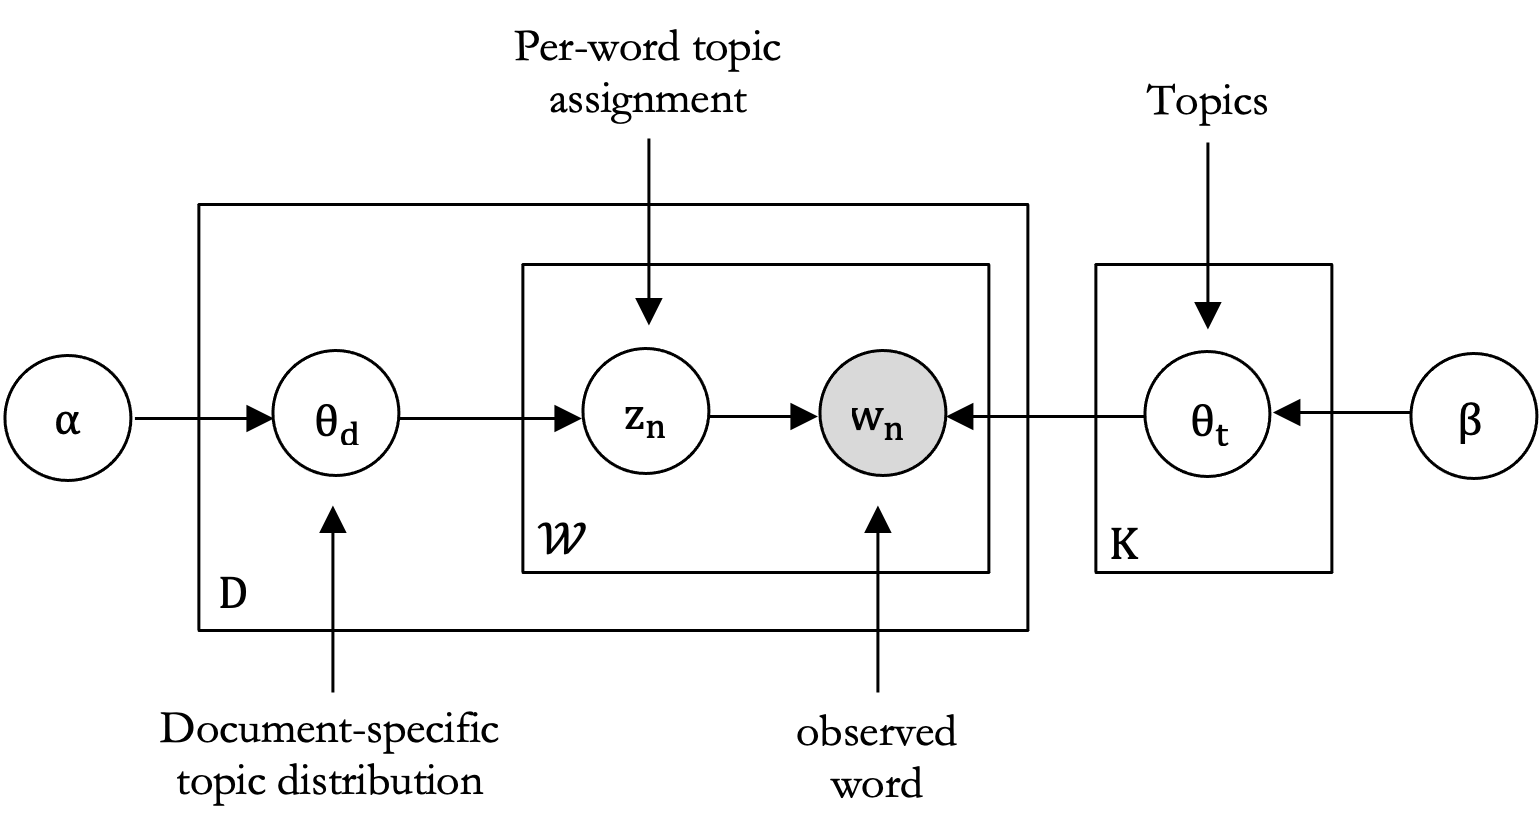
\includegraphics[width=\textwidth]{gfx/LDA_model}
  \caption{Graphical representation of \ac{LDA}}
  \label{fig:4-LDA}
\end{figure}

A topic found in a document $d_i$ is usually shown as a combination of a word $w_i$ and its probability $p_i$ in the distribution $\phi_i$, as $(p_i \ast w_i)$. For example, $(fact \ast 0.01)$ or $(fake \ast 0.001)$. Each topic distribution contains the entire vocabulary, with varying probabilities assigned to each word. The word with the highest probability in the distribution is usually used to label a topic.\sidecite{Maiya:2015} Words that have higher probabilities within a topic would tend to co-occur in the corpus as a whole.

\ac{LDA} generates document-topic distributions $\theta_d$ and word-topic distributions $\phi_t$. \autoref{fig:4-LDA}\sidenote{Adapted from \citeauthoryear{Blei:2003} (Fig. 1) and \citeauthoryear{Blei:2012} (Fig. 4).} shows a graphical model of \ac{LDA}. The box labelled $D$ represents the documents in a corpus. While boxes $\mathscr{W}$ and $K$ represent the repeatedly selected words and topics within a document, respectively. The circles are random variables in the generative process. The Dirichlet parameter $\alpha$  controls the sparsity of topics within documents, while $\beta$ controls the sparsity of words within topics. The hidden variables (topics, topic proportions, and assignments) are unshaded, while the observed variable (words in a document) is shaded.

\subsection{Distance measures}
\label{ssec:4-LDA}

Distributional similarity/distance measures are commonly used to compare the similarities, differences and overlaps between topics extracted from corpora.\sidenote{\citeauthoryear{Omar:2015}, \citeauthoryear{Vosoughi:2018}}

All articles $S_{bg}$ are split into two parts: its first $x$ sentences\sidenote{Only articles with at least $x + 1$ sentences are used.}, and the remaining $y$. Next, $N$ topics are obtained from $x$ and $y$ from an \ac{LDA} model trained on the entire dataset. For $i = (1, \ldots, m)$ topics, let $p_x = (p_{x1}, \ldots, p_{xm})$ and $p_y = (p_{y1}, \ldots, p_{ym})$ be two vectors of topic distributions, which denote the prevalence of a topic $i$ in the opening text $x$ and remainder $y$ of an article, respectively. Finally, the average and median values of each distance are calculated across all fake ($S_f$) and real ($S_r$) articles. These steps were repeated with varying values of $N$ (from 10 to 200 topics) and $x$ (from 1 to 5 sentences).

The following are the data required for this procedure: a corpus $S_{bg} = S_f \bigcup S_r$ of full-length fake ($S_f = \left\{ d_1^f, d_2^f, \ldots, d_F^f \right\}$) and real ($S_r = \left\{ d_1^r, d_2^r, \ldots, d_R^r \right\}$) documents.

The following measures were considered for calculating the topical divergence between parts $x$ and $y$ of an article:

\begin{enumerate}
  \item \underline{Cosine distance ($D_{C}$)}:
    \begin{equation} \label{eq:4-dc}
    D_{C}\left( p_x, p_y \right) = \frac{p_x \cdot p_y}{\big\| p_x \big\| \: \big\| p_y \big\|} = 1 - \frac{\sum _{i=1}^{m}  p_{x_i} p_{y_i} }{ \sqrt{\sum _{i=1}^{m} {p_{x_i}}^2 } \: \sqrt{\sum _{i=1}^{m} {p_{y_i}}^2} }
    \end{equation}

  \item \underline{Chebyshev distance ($D_{Ch}$)}:
    \begin{equation} \label{eq:4-dch}
    D_{Ch}\left( p_{x_i}, p_{y_i} \right) = \underset{i = 1 \ldots m}{\max} \: \left| p_{x_i} - p_{y_i} \right|
    \end{equation}

  \item \underline{Euclidean distance ($D_E$)}:
    \begin{equation} \label{eq:4-de}
    D_E\left( p_{x_i}, p_{x_i} \right) = \norm{p_{x_i} - p_{x_i}} = \sqrt {\sum _{i=1}^{m} \left( p_{x_i} - p_{x_i} \right)^2 }
    \end{equation}

  \item \underline{Hellinger distance ($D_{H}$)}:
    \begin{equation} \label{eq:4-dh}
    D_{H}\left( p_x, p_y \right) = \frac{1}{\sqrt{2}}\sqrt{\sum _{i=1}^{m} { \left( \sqrt{p_{x_i}} - \sqrt{p_{y_i}} } \right) ^2}
    \end{equation}

  \item \underline{Jensen-Shannon divergence ($D_{JS}$)}:
    \begin{equation} \label{eq:4-djs}
    D_{JS}\left( p_x \: \big\| \: p_y \right) = \frac{1}{2} \left[ D_{KL}\left( p_x \: \big\| \: p_z \right) + D_{KL}\left( p_y \: \big\| \: p_z \right) \right]
    \end{equation}
    where $p_z = \frac{1}{2} \left( p_x + p_y \right) $

  \item \underline{Kullback-Leibler (KL) divergence ($D_{KL}$)}\sidenote{$D_{KL}$ is not symmetric and therefore not a metric, but it can be transformed into one—to form the Jensen-Shannon divergence, $D_{JS}$ (\autoref{eq:4-djs}).
  }:
    \begin{equation}
    D_{KL}\left( p_x \: \big\| \: p_y \right) = \sum_{i=1}^{m} p_{x_i} \log{\frac{p_{x_i}}{p_{y_i}}}
    \end{equation}

  \item \underline{Squared Euclidean distance ($D_{SE}$)}:
    \begin{equation}
      D_E\left( p_{x_i}, p_{x_i} \right) = \norm{p_{x_i} - p_{x_i}}^2 = \sum _{i=1}^{m} \left( p_{x_i} - p_{x_i} \right)^2
    \end{equation}
\end{enumerate}

These measures were all used in the preliminary explorations carried out for this chapter. Eventually, however, only three ($D_Ch$, $D_{E}$, and $D_{SE}$) were proceeded with in the main experiments. Intuitively, the cosine distance indicates the \emph{angular} gap between two vectors (distributions of topics, in this case). Chebyshev distance is the greatest difference found between any two topics in $x$ and $y$. The Euclidean distance measures how \emph{far} the two topic distributions are from one another, while the Squared Euclidean distance is simply the square of that \emph{farness}. The other measures ($D_H$, $D_{JS}$, and $D_{KL}$) were considered as they were originally developed to deal directly with probability distributions.

\begin{algorithm}
\caption{Evaluation of thematic divergence in news articles}\label{4-divergence}
\begin{algorithmic}[1]

\Require
  {\begin{minipage}[t]{10cm}%
     \strut
     (i.) Pairs of first $l = [1, 2, \ldots, 5]$ sentences and remainder $y$ of each fake ($d_i^f = \left\langle d_{i_x}^f, \: d_{i_y}^f \right\rangle $; $ \left| d_{i_x}^f \right| = l$) and real article ($d_i^r = \left\langle d_{i_x}^r, \: d_{i_y}^r \right\rangle $; $ \left| d_{i_x}^r \right| = l$);

     (ii.) \ac{LDA} model $\mathscr{M}_{bg}$ generated using $S_{bg}$;

     (iii.) Number of topics $N \in \{ 10, 20, 30, 40 50, 100, 150, 200 \}$;

     (iv.) Divergence function $\mathscr{D} \in \{ D_{Ch}, D_E, D_{SE} \}$
     \strut
   \end{minipage}%
  }

\Ensure $ \left\{ D_{avg}^f, D_{avg}^r, D_{med}^f, D_{med}^r \right\}$
\item[]
\ForAll {$l = [1, 2, \ldots, 5]\ $}
  \ForAll {fake articles $ \left\langle d_{i_x}^f, \: d_{i_y}^f \right\rangle $}
    \State get $N$ topics in $d_{i_x}^f$ and $d_{i_y}^f$ using $\mathscr{M}_{bg}$
  \EndFor
  \State $T_{i_x}^f = \left( p_i^x, \ldots, p_N^x \right)^f$ \Comment{Topics in opening of fake article}
  \State $T_{i_y}^f = \left( p_i^y, \ldots, p_N^y \right)^f$ \Comment{Topics in remainder of fake article}
  \State $ D_i^f = \mathscr{D} \left( T_{i_x}^f, T_{i_y}^f \right) $
  \ForAll {real articles $ \left\langle d_{i_x}^r, \: d_{i_y}^r \right\rangle $}
    \State get $N$ topics in $d_{i_x}^r$ and $d_{i_y}^r$ using $\mathscr{M}_{bg}$
  \EndFor

  \State $T_{i_x}^r = \left( p_i^x, \ldots, p_N^x \right)^r$ \Comment{Topics in remainder of real article}
  \State $T_{i_y}^r = \left( p_i^y, \ldots, p_N^y \right)^r$ \Comment{Topics in remainder of real article}
  \State $ D_i^r = \mathscr{D} \left( T_{i_x}^r, T_{i_y}^r \right) $

  \State $D_{avg}^f = mean \left( \left.D_i^f\,\right\vert_{i \in \{1, \ldots, F\}} \right) $; \: $D_{avg}^r = mean \left( \left.D_i^r\,\right\vert_{i \in \{1, \ldots, R\}} \right) $

  \State $D_{med}^f = median \left( \left.D_i^f\,\right\vert_{i \in \{1, \ldots, F\}} \right) $; \: $D_{med}^r = median \left( \left.D_i^r\,\right\vert_{i \in \{1, \ldots, R\}} \right) $
\EndFor

\State\Return $ \left\{ D_{avg}^f, D_{avg}^r, D_{med}^f, D_{med}^r \right\}$
\end{algorithmic}
\end{algorithm}

\section{Experiment}
\label{sec:4-experiment}

\subsection{Preprocessing}
\label{ssec:4-preprocessing}

All computational operations in this experiment were performed using Python and freely available packages. Preprocessing for each dataset was done in the following steps:

\begin{enumerate}
  \item Articles are split into sentences using the \texttt{NTLK}\sidenote{\raggedright\url{https://www.nltk.org}} package. Each sentence is tokenised, lowercased and normalised (\emph{i.e.}, accentuations are removed) to form a list of words, from which stopwords are removed. The union of the built-in stopwords in the \texttt{NLTK}  and \texttt{spaCy} toolkits, as well as the MySQL Reference Manual,\sidenote{\raggedright\url{https://dev.mysql.com/doc/refman/8.0/en/fulltext-stopwords.html}} was used to filter irrelevant words. Furthermore, additional words typically found in news text but can be considered to be unimportant were added. Examples of such words include long and short forms of days of the week, and months, and others such as \emph{`says'}, \emph{`said'}, \emph{`Reuters'}, \emph{`Mr'}, and \emph{`Mrs'}.

  \item Bigrams were created from two consecutive words which appeared several times in the corpus. A minimum count of such instances was set to five and a threshold score as explained in \citeauthoryear{Mikolov:2013b} of 100 was used. The bigrams are then added to the vocabulary.

  \item Next, each document is lemmatized using \texttt{spaCy}\sidenote{\raggedright\url{https://spacy.io/models/en}}, and only noun, adjective, verb, and adverb lemmas are retained. A dictionary is formed by applying these steps to $S_{bg}$.

  \item Each document is converted into a \ac{BoW} format,\sidenote{\raggedright A list of (\texttt{token\_id}, \texttt{token\_count}) tuples.} which is used to create an \ac{LDA} model $\mathscr{M}_{bg}$. The models were created with \texttt{Gensim}.\sidenote{\raggedright\url{https://radimrehurek.com/gensim}}

  \item Fake and real articles are subsequently preprocessed likewise (\emph{i.e.}, from raw text data to \ac{BoW} format) before topics are extracted from them.
\end{enumerate}

Although there is no consensus on whether the inclusion or omission of stopwords yields better topic models,\sidecite{Shi:2019} stopwords can affect the interpretability of topics as they can diminish the appearance of other more important words. In this experiment, the goal is to find differences between topics extracted from legitimate and false news. As false news content often cunningly mimics true news, it is important to remove words which are contextually irrelevant and focus on words which can help us tell the two apart.

\subsection{Datasets}
\label{ssec:4-datasets}

\autoref{tab:4-datasets} summarizes the datasets (after preprocessing) used in this study and lists the domains (as stated by the dataset provider) covered by each. An article’s sentence length (Avg. sent. length) is measured by the number of words that remain after preprocessing. The article's maximum sentence length (Max. sent length) is measured in terms of the number of sentences. The following datasets were used:

\begin{enumerate}
  \item BuzzFeed-Webis Fake News Corpus 2016 (BuzzFeed-Web)\sidenote{\citeauthoryear{Potthast:2018}, \raggedright\url{https://zenodo.org/record/1239675}}
  \item BuzzFeed Political News Data (BuzzFeed-Political)\sidenote{\citeauthoryear{Horne:2017}, \raggedright\url{https://github.com/BenjaminDHorne/fakenewsdata1}}
  \item FakeNewsAMT + Celebrity (AMT+C)\sidecite{Perez-Rosas:2018}
  \item Falsified and Legitimate Political News Database  (POLIT)\sidenote{\raggedright\url{http://victoriarubin.fims.uwo.ca/news-verification/access-polit-false-n-legit-news-db-2016-2017}}
  \item George McIntire's fake news dataset (GMI)\sidenote{\raggedright\url{https://github.com/GeorgeMcIntire/fake_real_news_dataset} (Accessed 5 November 2018)}
  \item University of Victoria's Information Security and Object Technology (ISOT) Research Lab\sidenote{\citeauthoryear{Ahmed:2017}, \raggedright\url{https://www.uvic.ca/engineering/ece/isot}}
  \item Syrian Violations Documentation Centre (SVDC)\sidenote{\citeauthoryear{AbuSalem:2019}, \raggedright\url{https://zenodo.org/record/2532642}}
\end{enumerate}

\newpage
\begin{table}[h]
\addlinespace
    \begin{tabularx}{480pt}{>{\raggedright}p{3.5cm}llllll}
      \toprule
        \tableheadline{\shortstack[l]{Dataset \smallskip\\ (domain)}} &

        \tableheadline{\shortstack[l]{No. of \smallskip\\ fake}} &

        \tableheadline{\shortstack[l]{No. of \smallskip\\ real}} &

        \tableheadline{\shortstack[l]{Avg. sent \smallskip\\ length (f)}} &

        \tableheadline{\shortstack[l]{Avg. sent \smallskip\\ length (r)}} &

        \tableheadline{\shortstack[l]{Max. sent \smallskip\\ length (f)}} &

        \tableheadline{\shortstack[l]{Max. sent \smallskip\\ length (r)}} \\

      \midrule
        AMT+C\\ (business, education, entertainment, politics, sports, tech) & 324 & 317 & 14.7 & 23.2 & 64 & 1,059 \\

        BuzzFeed-Political\\ (politics) & 116 & 127 & 18.9 & 43.9 & 76 & 333 \\

        BuzzFeed-Web\\ (politics) & 331 & 1,214 & 21.7 & 26.4 & 117 & 211 \\

        GMI\\ (politics) & 2,695 & 2,852 & 33.9 & 42.8 & 1,344 & 406 \\

        ISOT\\ (government, politics) & 19,324 & 16,823 & 18.0 & 20.3 & 289 & 324 \\

        POLIT\\ (politics) & 122 & 134 & 19.2	& 34.9 & 96 & 210 \\

        SVDC\\ (conflict, war) & 312 & 352 & 14.0 & 14.6 & 62 & 49 \\
        \bottomrule
    \end{tabularx}
\caption{Summary of datasets after pre-processing (F – Fake, R – Real).}
\label{tab:4-datasets}
\end{table}

\section{Results and discussion}
\label{sec:4-results-discussion}

As can be seen in the first line of Algorithm \autoref{4-divergence}, experimented with were varying values of hyperparameter for the length of the opening section, $l$, from 1 to 5. Results for $l=5$ are reported in this section because during initial analyses it yielded the best results (\emph{i.e.}, the greatest disparity between fake and real deviations) for most datasets and measures. This is likely due to the first five sentences containing more information. For example, five successive sentences are likely to entail one another and contribute more towards a topic than a single sentence.

The outcomes of the experimental evaluation using the different divergence measures are shown in \autoref{tab:4-results-ttest}.\sidenote{The average of each $N$ group was found before doing the T-test.} It was observed that fake news is generally likely to show greater thematic deviation (lesser coherence) than real news in all datasets. Nonetheless, the mean and median values for fake news are lower than those of real news for these datasets. \autoref{tab:4-results-mean-median}, shows the mean and median $D_{Ch}$ deviations of fake and real articles across all values of $N$, while \autoref{fig:4-results} shows results for comparing topics in the first five and remaining sentences. Results for values of $N$ not shown are similar (with $D_{Ch}$ gradually decreasing as $N$ increases).

As the results for all three measures are alike, $D_{Ch}$ is focused on for the rest of the analysis. This is because the choice of divergence measure is not critical to the outcome of the experiment. Rather it is only a means for estimating thematic divergence. \autoref{tab:4-results-mean-median} shows the mean $D_{Ch}$ deviations of fake and real articles across $N = \{ 10, 20, 30, 40, 50, 100, 150, 200 \} $ topics.

AMT+C and BuzzFeed-Web are not statistically significant according to the T-test. However, the results for all other datasets are. Therefore, for all datasets except AMT+C and BuzzFeed-Web, the null hypothesis (\Cref{hyp:a})—that false and authentic news articles are similarly coherent thematically—is rejected at the 5\% level, based on the T-test. In summary, it has been shown statistically that thematic coherence is generally greater in real news articles compared to fake ones.

\begin{table}[h]
\addlinespace
    \begin{tabularx}{\textwidth}{>{\raggedright}p{3.5cm}lll}
      \toprule
        \tableheadline{Dataset} &
        \tableheadline{p-value ($D_{Ch}$)} &
        \tableheadline{p-value ($D_{E}$)} &
        \tableheadline{p-value ($D_{SE}$)} \\
      \midrule
        AMT+C & 0.144 & 0.126	& 0.116 \\
        BuzzFeed-Political & 0.0450 & 0.0147 &	0.0287 \\
        BuzzFeed-Web & 0.209 & 0.209 &	0.207 \\
        GMI & 0.0480 & 0.00535 & 0.0106 \\
        ISOT & 0.00319 & 0.000490	& 0.000727 \\
        POLIT & 0.000660 & 0.0000792 & 0.0000664 \\
        SVDC & 0.000684	& 0.0000112 &	0.0000789 \\
      \bottomrule
    \end{tabularx}
\caption{Results of T-test evaluation based on different measures of deviation used.}
\label{tab:4-results-ttest}
\end{table}

\begin{table}[h]
\addlinespace
    \begin{tabularx}{480pt}{>{\raggedright}p{3.5cm}llll}
      \toprule
        \tableheadline{Dataset} &
        \tableheadline{Mean ($D_{Ch}$) (F)} &
        \tableheadline{Mean ($D_{Ch}$) (R)} &
        \tableheadline{Median ($D_{Ch}$) (F)} &
        \tableheadline{Median ($D_{Ch}$) (R)} \\
      \midrule
        AMT+C & 0.2568 & 0.2379	& 0.2438 & 0.2285 \\
        BuzzFeed-Political & 0.2373	& 0.2149 & 0.2345 & 0.2068 \\
        BuzzFeed-Web & 0.2966 & 0.2812 & 0.2863 & 0.2637 \\
        GMI & 0.4580 & 0.4241	& 0.4579 & 0.4222 \\
        ISOT & 0.3372	& 0.2971 & 0.3369 & 0.2989 \\
        POLIT & 0.2439 & 0.1939	& 0.2416 & 0.1894 \\
        SVDC & 0.2975 & 0.2517 & 0.2934 & 0.2435 \\
      \bottomrule
    \end{tabularx}
\caption{Mean and median $D_{Ch}$ deviations of $N = \{ 10, 20, 30, 40, 50, 100, 150, 200 \} $ topics combined for fake and real news (F – Fake, R – Real).}
\label{tab:4-results-mean-median}
\end{table}

\begin{figure}[th]
    \centering
    \begin{subfigure} %1
        \subfloat[Results for AMT+C]
        {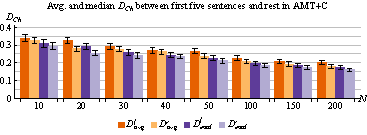
\includegraphics[width=480pt]{gfx/4_AMTC}}
        \label{fig:4-results-amtc}
    \end{subfigure}

    \begin{subfigure} %2
        \subfloat[Results for BuzzFeed-Political]
        {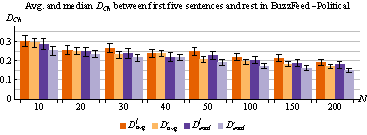
\includegraphics[width=480pt]{gfx/4_BP}}
        \label{fig:4-results-bp}
    \end{subfigure}

    \begin{subfigure} %3
        \subfloat[Results for BuzzFeed-Web]
        {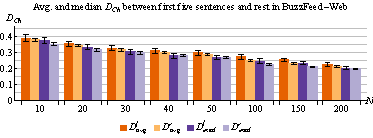
\includegraphics[width=480pt]{gfx/4_BW}}
        \label{fig:4-results-bw}
    \end{subfigure}

    \caption{Average and median Chebyshev distances in fake and real news, when comparing topics in the first five sentences to the rest of each article. Error bars show 95\% confidence interval.}\label{fig:4-results}
\end{figure}

\begin{figure}[th]\ContinuedFloat
    \centering
    \begin{subfigure} %4
        \subfloat[Results for GMI]
        {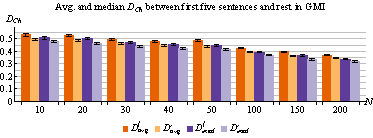
\includegraphics[width=480pt]{gfx/4_GMI}}
        \label{fig:4-results-gmi}
    \end{subfigure}

    \begin{subfigure} %5
        \subfloat[Results for ISOT]
        {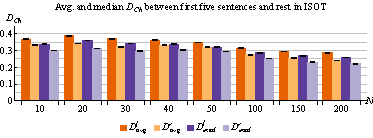
\includegraphics[width=480pt]{gfx/4_ISOT}}
        \label{fig:4-results-isot}
    \end{subfigure}

    \begin{subfigure} %6
        \subfloat[Results for POLIT]
        {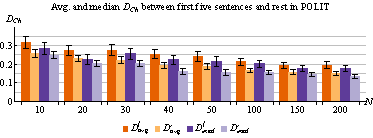
\includegraphics[width=480pt]{gfx/4_POLIT}}
        \label{fig:4-results-polit}
    \end{subfigure}

    \caption{Average and median Chebyshev distances in fake and real news, when comparing topics in the first five sentences to the rest of each article. Error bars show 95\% confidence interval. (Cont.)}\label{fig:4-results}
\end{figure}

\begin{figure}[th]\ContinuedFloat
    \centering
    \begin{subfigure} %7
        \subfloat[Results for SVDC]
        {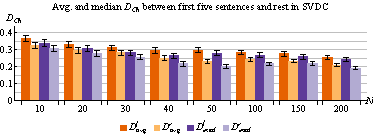
\includegraphics[width=480pt]{gfx/4_SVDC}}
        \label{fig:4-results-svdc}
    \end{subfigure}
    \caption{Average and median Chebyshev distances in fake and real news, when comparing topics in the first five sentences to the rest of each article. Error bars show 95\% confidence interval. (Cont.)}\label{fig:4-results}
\end{figure}
\FloatBarrier

It is worth highlighting the diversity of datasets used here, in terms of domain, size, and the nature of articles. For example, the fake and real news in the SVDC dataset have a very similar structure. Both types of news were mostly written with the motivation to inform the reader of conflict-related events that took place across Syria. However, fake articles are labelled as such primarily because the reportage (\emph{e.g.}, on locations and the number of casualties recorded) in them is insufficiently accurate.

\newthought{To gain insight} into possible causes of greater deviation in fake news, the five most and least diverging fake and real articles (according to $D_{Ch}$) were qualitatively inspected. A small set of low and high numbers of topics ($N \leq 30$ and $N \geq 100$) were also compared. It was observed that fake openings tend to be shorter, vaguer, and less congruent with the rest of the text. By contrast, real news openings generally give a better narrative background to the rest of the story. \citeauthoryear{Horne:2017} reported similar findings regarding the comparison in length, between authentic and false news articles: \emph{i.e.}, the former is generally longer than the latter, as shown in \autoref{tab:4-datasets}. Furthermore, the same study also found that fake articles are highly redundant and contain less substantial information.

Although the writing style in fake news is sometimes unprofessional, this is an unlikely reason for the higher deviations in fake news. Additionally, both fake and real news may open with the most newsworthy content, and expand on it with more context and explanation. This is the conventional hierarchical structure of news,\sidecite{Dijk:1983} as discussed in \sectionref{sec:2-existing}.

Indeed, in this study, it was observed that real news tends to have longer sentences, which give more detailed information about a story and are more narrative. It can be argued that the reason behind this is that fake articles are designed to get readers’ attention, whereas legitimate ones are written to inform the reader. For instance, social media posts which include a link to an article are sometimes displayed with a short snippet of the article’s opening text or its summary. This section can be designed to capture readers’ attention.

It was also observed that fake articles include more question and exclamation marks, as well as words and phrases in all capitals. Although this is inconsequential to forming topics, it supports the claim that false news is written in an attention-grabbing style. While \citeauthoryear{Horne:2017} state that punctuation is less likely to be found in fake news text, \citeauthoryear{Rubin:2016} suggest that it is a differentiating factor between fake and real news. Punctuation marks, including question and exclamation marks, have also been used as a feature in fake news detection.\sidecite{Perez-Rosas:2018}

Furthermore, it is conceivable that a bigger team of people working to produce a fake piece may contribute to its vagueness. They may input different perspectives that diversify the story and make it less coherent. This may be compared with real news, whereby there is one professional writer, perhaps two, and therefore, better coherence.

\subsection{Quantitative analysis of coherence and perplexity}
\label{ssec:4-coherence-perplexity}

The observation of greater thematic deviation was further explored experimentally. The qualitative findings previously discussed can be more reliably verified through quantitative analyses, using empirical measures for \emph{topic coherence}.\sidenote{This should not be confused with the concept of \emph{thematic coherence} earlier introduced in this chapter. Whereas the former is used in this thesis to denote consistency in the subject(s) discussed throughout a news article, the latter is a measure for evaluating topics in general.}

Topic coherence assigns a score to each topic by evaluating the semantic similarity between top words in the topic.\sidecite{Stevens:2012} It is capable of reflecting people’s perception of latent topics in a given text.\sidecite{Blair:2019} Thus, topic coherence is adopted here as an \emph{indicator} of the amount of vagueness in an article. The intuition behind this is that topics with high coherence constitute words which allow a reader to infer the general topic(s) the text is about. Conversely, those with very low coherence are hardly interpretable,\sidecite{Roder:2015} and hence, are likely to arise from vaguer text.

Topic coherence measures fall into two groups:
\begin{enumerate}
  \item Intrinsic measures, which capture model semantics and are based on human evaluation of topics’ interpretability.
  \item Extrinsic measures, which indicate how good a topic model is at performing predefined tasks such as classification.
\end{enumerate}

As intrinsic measures are based on human evaluations, they are more apt for indicating how a person might assess the coherence of an article they are reading. Moreover, intrinsic measures have been shown to correlate better with human judgement.\sidecite{Chang:2009} Therefore, one such measure called UMass\sidecite{Mimno:2011} is used. This is defined in \autoref{eq:4-umass} as was done by \citeauthoryear{Stevens:2012}. From a set of top words used to describe a topic, UMass measures the extent to which a common word is a good predictor of a less common word on average.\sidenote{\citeauthoryear{Mimno:2011}, \citeauthoryear{Hemmatian:2019}}

\begin{equation} \label{eq:4-umass}
score_{UMass}\left( v_i, v_j, \epsilon \right) = log \: \frac{ D\left( v_i, v_j \right) + \epsilon }{ D\left(v_j\right) }
\end{equation}
\begin{conditions}
 D(x)        &  number of documents which contain word $x$\\
 D(x, y)     &  number of documents containing words $x$ and $y$\\
 \epsilon    &  smoothing factor that ensures $score_{UMass}$ is a real number
\end{conditions}

Topic coherence was evaluated in two ways: (i.) the openings of fake ($S1$) and authentic articles ($S2$); and (i.) the whole articles. In both cases, the numbers of topics ($N$) studied are $10, 20, \ldots, 140, 150, 200$.\sidenote{Note that a wider range of $N$ is used here, compared with Algorithm \autoref{4-divergence}.}


% ————————————————————————————————
%
\newthought{$S2$ articles in} the AMT+C dataset have greater coherence than $S1$ ones. This becomes more apparent when $N \geq 40$. However, focusing on the opening sections, it can be seen that $S1$ opening sentences are only slightly more coherent than $S2$ ones. This means that although $S2$ in this dataset are more topically coherent, the opening sections of $S1$ are more coherent.

In the BuzzFeed dataset, it can be seen that $S2$ articles are more coherent than $S1$ articles, both for opening and whole texts. For the openings in BuzzFeed Political, $S2$ articles are only slightly more coherent. Nonetheless, whole $S2$ articles are noticeably more coherent than $S1$ articles. Considering the opening sections, it is clear that the $S2$ coherence scores are generally—though only marginally in most cases—higher than those of $S1$.

\autoref{fig:4-umass-coherence} shows UMass scores for the first five sentences of $S1$ and $S2$ articles, calculated over the training set (a combination of all $S1$ and $S2$ full articles). Higher values indicate higher topic coherence, \emph{i.e.}, words associated with each topic in that model are more likely to co-occur. As expected, more topics are generally less coherent than fewer ones.

\begin{figure}[ht]
    \centering

    \subfloat[\centering ]{
    \begin{minipage}{240pt}{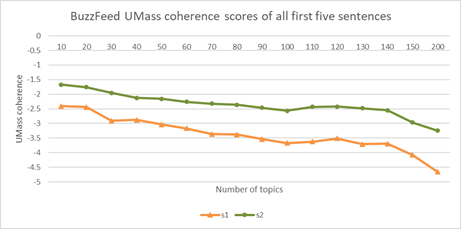
\includegraphics[width=230pt]{gfx/4_umass_amt+C} }
    \end{minipage}
    }
    \subfloat[\centering ]{
    \begin{minipage}{240pt}{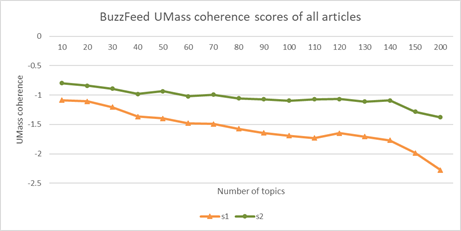
\includegraphics[width=230pt]{gfx/4_umass_amt+C_2} }
    \end{minipage}
    }

    \subfloat[\centering ]{
    \begin{minipage}{240pt}{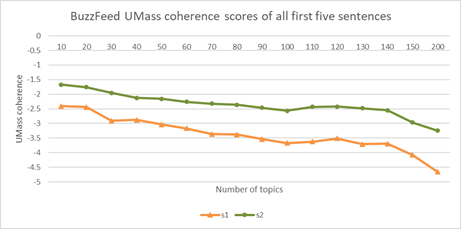
\includegraphics[width=230pt]{gfx/4_umass_bf} }
    \end{minipage}
    }
    \subfloat[\centering ]{
    \begin{minipage}{240pt}{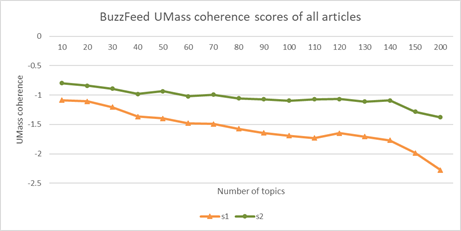
\includegraphics[width=230pt]{gfx/4_umass_bf_2} }
    \end{minipage}
    }
\end{figure}

\begin{figure}[ht]
    \ContinuedFloat \centering

    \subfloat[\centering ]{
    \begin{minipage}{240pt}{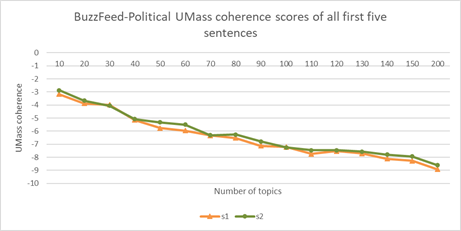
\includegraphics[width=230pt]{gfx/4_umass_bfp} }
    \end{minipage}
    }
    \subfloat[\centering ]{
    \begin{minipage}{240pt}{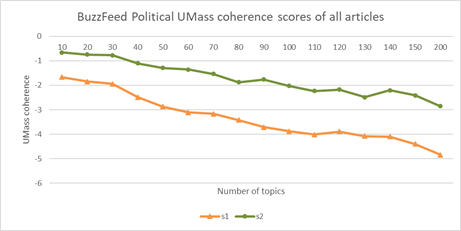
\includegraphics[width=230pt]{gfx/4_umass_bfp_2} }
    \end{minipage}
    } \medskip

    \subfloat[\centering ]{
    \begin{minipage}{240pt}{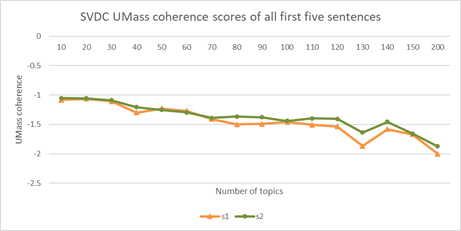
\includegraphics[width=230pt]{gfx/4_umass_svdc} }
    \end{minipage}
    }
    \subfloat[\centering ]{
    \begin{minipage}{240pt}{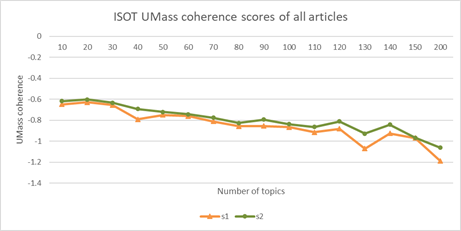
\includegraphics[width=230pt]{gfx/4_umass_svdc_2} }
    \end{minipage}
    }

    \centering
    \caption{UMass topic coherence scores}
    \label{fig:4-umass-coherence}
\end{figure}
\FloatBarrier
%
% ————————————————————————————————


\newthought{In summary, the} topic coherence of authentic news is generally greater than that of misinformation, in all datasets except AMT+C. This is the case in the articles' opening sections, and when considering the whole article. The UMass coherence scores suggest that true articles are less vague, compared with fake ones, as they form more coherent topics. This corroborates earlier qualitative findings on the coherence of real and fake articles. Nonetheless, manual inspection of the top words in each topic may still be required. While some datasets show a clear distinction between false and true articles’ coherence scores, the disparity is not clear in others.

Ideally, applying insights from \citeauthoryear{Roder:2015}, a different topic coherence score called $C_V$, should be used. The authors found this to be the best amongst topic coherence measures in their study. The $C_V$ score uses Normalized Pointwise Mutual Information and cosine similarity measure (see \autoref{eq:4-dc}) in its workings. One drawback of the $C_V$ score is its runtime—it takes more than twenty times longer to run compared with UMass. In any case, the performance of UMass suffices in this exploration.

The datasets analysed here cover a broad range of themes and contain articles with different structures and writing styles. Furthermore, their constituent false and real articles have sentences of varying lengths and vocabularies of varying sizes. These findings show that regardless of the individual attributes of datasets, fake news articles appear to have some high-level features which can be used to systematically tell them apart from real news.

\section{Conclusion}
\label{sec:4-conclusion}

Fake news and deceptive stories tend to open with sentences which may be incoherent with the rest of the text. It is worth exploring if the consistency of fake and real news can distinguish between the two. Accordingly, the thematic deviations of seven cross-domain fake and real news, using topic modelling were investigated. The findings presented in this chapter suggest that the opening sentences of fake articles topically deviate more from the rest of the article, in contrast to real news. The next step is to find possible reasons behind these deviations through in-depth analyses of topics. In conclusion, this paper presents valuable insights into thematic differences between fake and authentic news, which may be exploited for fake news detection.

\subsection{Future work}
\label{ssec:4-future-work}

Future work can extend this research in two main ways. Firstly, experimenting with topic modelling methods other than \ac{LDA} may improve the results. One example that has been demonstrated to outperform \ac{LDA} in the task of learning insightful topics is \texttt{top2vec}\sidecite{Angelov:2020}. This topic modelling algorithm combines document and word vectors to find topics. Both are commonly used features for fake news detection. With \texttt{top2vec}, topic vectors are indicative of the semantic similarity between documents. Additionally, it automatically finds the optimal number of topics. By comparison, this is done iteratively with \ac{LDA}, by evaluating metrics such as \emph{perplexity} across a varying number of topics.

Secondly, other techniques beyond splitting an article into multiple parts can also be investigated. Ideally, the feature extraction method should be resilient to minor alterations in the news text. It is worth stating that experiments in parallel with this idea were also carried out in this research. For example, the semantic coherence between the extractive summaries and opening paragraphs of articles was evaluated, using word embeddings obtained from \ac{BERT}.\sidecite{Devlin:2019} Further experiments were carried out to find the amount of overlap between the summaries and opening paragraphs, and the positions of sentences in each article, which constitute its extractive summary. This branch of experiments did not show semantic coherence—found in this particular way—to be a robust marker of misinformation detection. Nonetheless, it can be further investigated in future research.

% end of chapter
